\chapter{Methodology} 
\label{chapter:method}

\pagestyle{plain}
% Define some numbers here for the autmation of the tables
\newcommand{\libsodiumfunctions}{869}
\newcommand{\qrcodefunctions}{1849}
\newcommand{\allmewefunctions}{\libsodiumfunctions + \qrcodefunctions}

% Execute a python script for small calculations
\newcommand{\py}[1]{\input{|python3 interpreter.py #1}}
\newcommand{\fromjson}[2]{\input{| jq -r '#2' #1}}

\newcommand{\corpusrosetta}{\fromjson{data/crow_corpus.json}{.[0].name}}
\newcommand{\corpussodium}{Libsodium\xspace}
\newcommand{\corpusqrcode}{QrCode\xspace}


\newcommand{\DTWStatic}{dt\_static\xspace}
\newcommand{\DTW}{dt\_dyn\xspace}
\newcommand{\tool}{CROW\xspace}


%This chapter investigates whether we can artificially create program variants through semantically equivalent code transformations. We propose a framework to generate program variants functionally equivalent to their original.
%We introduce the retargeting of a superoptimizer, using its exhaustive search strategy to provide semantically equivalent code transformations. 
%The presented methodology and transformation tool, CROW, are contributions to this thesis.
%We evaluate the usage of CROW on two corpora of open-source and nature diverse programs. 
In this chapter, we present our methodology to answer the research questions enunciated in \autoref{intro:definition:rq}.
We investigate three research questions. In the first question, we artificially generate \wasm program variants and quantitatively compare the static differences between variants. 
Our second research question focuses on comparing their behavior during their execution.
The final research question evaluates the feasibility of using the program variants in security-sensitive environments such as Edge-Cloud computing proposing a multivariant execution approach.

The main objective of this thesis is to study the feasibility of automatically creating program variants out of preexisting program sources. To achieve this objective,
we use an empirical method \cite{Runeson2020}, proposing a solution and evaluating it through quantitative analyzes in case studies. We follow an iterative and incremental approach on the selection of programs for our corpora. To build our corpora, we find a representative and diverse set of programs to generalize, even when it is unrealistic following an empirical approach, as much as possible our results.
We first enunciate the corpora we share along this work to answer our research questions. Then, we establish the metrics for each research question, set the configuration for the experiments, and describe the protocol.

% Our approach lies under \textit{Design Science} \cite{Runeson2020}, in terms of empirical validation, the scope of the design knowledge gained in a study can be extended by systematically extending the scope of the valudation in subsequent studies. Thus, the size of our corpora can be extended to increase the knowledge of the research area.


\section{Corpora}
\label{section:crow:corpora}

Our experiments assess the impact of artificially created diversity in terms of program variants size, static and dynamic differences. The first step is to build a suitable corpus of programs' seeds to generate the variants. Finally, we answer all our research questions with three corpora of diverse and representative programs for our experiments. 
We build our three corpora in an escalating strategy. The first corpus is diverse and contains simple programs in terms of code size, making them easy to analyze manually. The latter two corpora contain more extensive real-world programs, including one project meant for security-sensitive applications. Finally, all corpora are considered to come along the LLVM pipeline. We base this decision on the previous experimental work of Hilbig \etal \cite{Hilbig2021AnES}. This work shows that approximately 65\% of all \wasm programs come out of C/C++ source code, and more than 75\% if Rust is included. In the following, we describe the filtering and description of each corpus.

\begin{enumerate}
    \item \textbf{\corpusrosetta}: We take programs from the  Rosetta Code project\footnote{\url{http://www.rosettacode.org/wiki/Rosetta_Code}}. This website hosts a curated set of solutions for specific programming tasks in various programming languages. It contains many tasks, from simple ones, such as adding two numbers, to complex algorithms like a compiler lexer. We first collect all C programs from the Rosetta Code, representing $989$ programs as of 01/26/2020. We then apply several filters: the programs should successfully compile and, they should not require user inputs to automatically execute them, the programs should terminate and should not result in non-deterministic results. 
    
    The result of the filtering is a corpus of 303 C programs. All programs include a single function in terms of source code. These programs range from $7$ to $150$ lines of code and solve a variety of problems, from the \textit{Babbage} problem to  \textit{Convex Hull} calculation.

    \item \textbf{\corpussodium}: This project is encryption, decryption, signature, and password hashing library ported to WebAssembly in 102 separated modules. The modules have between $8$ and $2703$ lines of code per function. This project is selected based on two main criteria: first, its importance for security-related applications, and second, its suitability to collect the modules in LLVM intermediate representation. We select 5 programs that interconnect the 102 modules of the project.

    \item \textbf{\corpusqrcode}: This project is a QrCode and MicroQrCode generator written in Rust. This project contains 2 modules having between $4$ and $725$ lines of code per function. As \corpussodium, we select this project due to its suitability for collecting the modules in their LLVM representation. Besides, this project increases the complexity of the previously selected projects due to its integration with the generation of images.
    
\end{enumerate}

In \autoref{table:corpora} we listed the corpus name, the number of modules, the number of programs inside the corpus, the total number of functions, the range of lines of code, and the original location of the corpus. 


%The first corpus, \textbf{CROW prime}, . The second corpus, \textbf{MEWE prime}, is part of the MEWE contribution \cite{}. In \autoref{table:corpora} we summarize the selection criteria, and we mention each corpus properties. With both corpora we evaluate CROW with a total of $303 + \py{\allmewefunctions}$ functions. 

\begin{table}[h]
    \renewcommand{\arraystretch}{1.0}
    \small
    \centering
    \begin{tabular}{l | l | l | l | l | p{2.8cm}}
        Corpus & No. modules & No. programs & No. functions & LOC range & Location \\
        \midrule
            % CROW
            \corpusrosetta &
            - %\footnote{ The concept of module does not apply for this corpus programs. } 
            &
            \fromjson{data/crow_corpus.json}{.[0].programs} &
            \fromjson{data/crow_corpus.json}{.[0].functions}  & 
            \fromjson{data/crow_corpus.json}{.[0].min_lines} - 
            \fromjson{data/crow_corpus.json}{.[0].max_lines} & 
            \fromjson{data/crow_corpus.json}{.[0].url} \\
        \hline
        \corpussodium & 
        102 &
        5 & 
        \fromjson{data/allinone.multivariant.bc.massive.sodium.json}{.total_functions}  &
        \fromjson{data/allinone.multivariant.bc.massive.sodium.json}{.min_llvm_loc} - \fromjson{data/allinone.multivariant.bc.massive.sodium.json}{.max_llvm_loc}  &   
        \url{https://github.com/jedisct1/libsodium }\\
        \hline
        \corpusqrcode & 
        2 &
        2 & 
        \fromjson{data/allinone.multivariant.bc.massive.qr.json}{.total_functions}  & 
        \fromjson{data/allinone.multivariant.bc.massive.qr.json}{.min_llvm_loc} - \fromjson{data/allinone.multivariant.bc.massive.qr.json}{.max_llvm_loc}   & 
        \url{https://github.com/kennytm/qrcode-rust} \\
        % Total stats
        \hline
        \hline
        \textbf{Total} & 
        &
        \py{
        5 + 2 + 303} &   
        \py{ 303 + \qrcodefunctions + \libsodiumfunctions} &  
        &     \\

    \end{tabular}
    \caption{Corpora description. The table is composed by the name of the corpus, the number of modules, the number of programs, the number of functions, the lines of code range and the location of the corpus.}
    \label{table:corpora}
\end{table}


\section{\rqone}
\label{rq1:method}

\begin{figure}[h]
    \centering
    \includegraphics[height=4.1in]{diagrams/RQ1.pdf}
    \caption{The program variants generation for RQ1.}
    \label{diagrams:protocol:rq1}
\end{figure}


This research question investigates whether we can artificially generate program variants for \wasm. We use CROW to generate variants from an original program, written in C/C++ in the case of the \corpusrosetta corpus and LLVM bitcode modules in the case of the \corpussodium and \corpusqrcode. 
In \autoref{diagrams:protocol:rq1} we illustrate the workflow to generate \wasm\ program variants. We pass each function of the corpora to CROW as a program to diversify. To answer RQ1, we study the outcome of this pipeline, the generated \wasm\ variants. 


\subsection*{Metrics}

To assess our approach's ability to generate \wasm\ binaries that are statically different, we compute the number of variants and the number of unique variants for each original function of each corpus. 
On top, we define the aggregation of these former two values to quantitatively evaluate RQ1 at the corpus level. 

We start by defining what a program's population is. This definition can be applied in general to any collection of variants of the same program. All definitions are based upon bytecodes and not the source code of the programs.

\begin{definition}{Program's population $M(P)$:}\label{def:rq1:programspopulation}
    \normalfont 
    Given a program P and its generated variants $v_i$, the program's population is defined as:\\
    $$
        M(P)=\{v_i\ \text{where $v_i$ is a variant of P}\}
    $$

    Notice that the program's population includes the original program P.
\end{definition}

Beyond the program's population, we also want to compare how many program variants are unique. The subset of unique programs in the program's population hints how the variants are different between them and not only against the original program. For example, imagine a program $P$ with two program variants $V_1$ and $V_2$, the program population is composed by $\{P, V_1 \text{ and } V_2\}$, where $V_1$ is different from $P$, and $V_2$ is different from $P$. $V_1$ is either equal or different from $V_2$, the program's population still be the same. If $V_1$ and $V_2$ are equal, then only one unique variant is generated,

%\todo{
%   clarify source code versus byte code for earch definition.

%why are those definitions important? interesting? why do you introduce them?
%}
%Notice that all metrics over programs and their variants make sense only at the population level. Therefore, we compare semantically equivalent programs from the same population.

%\todo{
%   difference unclear or trivial.

%do you need source code versus bytecode?

%clarify
%}

\begin{definition}{Program's unique population $U(P)$:}\label{def:rq1:programsuniquepopulation}
    \normalfont 
    Given a program P and its program's population $M(P)$, the program's unique population is defined as.\\
    $$
        U(P)=\{v\ \in\ M(P)\}
    $$
    such that $\forall v_i,v_j \in U(P)$, $v_i \neg v_j$ $\Rightarrow$ $md5sum(v_i) \ne md5sum(v_j)$.
    $Md5sum(v)$ is the md5 hash calculated over the bytecode stream of the program file $v$. Notice that the original program $P$ is included in $U(P)$.

\end{definition}

\begin{metric}{Program's population size $S(P)$:}\label{metric:rq1:PS}
    \normalfont 
    Given a program P and its program's population $M(P)$ according to \autoref{def:rq1:programspopulation}, the program's population size is defined as.\\
    $$
        S(P)=|M(P)|
    $$
\end{metric}


\begin{metric}{Program's unique population size $US(P)$:}\label{metric:rq1:UP}
    \normalfont 
    Given a program P and its program's unique population $U(P)$ according to \autoref{def:rq1:programsuniquepopulation}, the program's unique population size is defined as.\\
    $$
        US(P)=|U(P)|
    $$
\end{metric}

\newcommand{\corpuspopulationsizename}{Corpus population size\xspace}
\newcommand{\corpusuniquepopulationsizename}{Corpus unique population size\xspace}

\begin{metric}{\corpuspopulationsizename$CS(C)$:}\label{metric:rq1:corpus_pop}
    \normalfont 
    Given a program's corpus $C$, the corpus population size is defined as the sum of all program's population sizes over the corpus $C$:\\
    $$
        CS(C)=\Sigma{S(P)}\ \forall\ P\ \in\ C
    $$
\end{metric}

\begin{metric}{\corpusuniquepopulationsizename$UCS(C)$:}\label{metric:rq1:corpus_pop_unique}
    \normalfont 
    Given a program's corpus $C$, the corpus unique population size is defined as the sum of all program's unique population sizes over the corpus $C$ :\\
    $$
    UCS(C)=\Sigma{US(P)}\ \forall\ P\ \in\ C
    $$
\end{metric}


\subsection*{Protocol}
To generate program variants, we synthesize programs with an enumerative strategy, checking each synthesis for equivalence modulo input \cite{Li2018} against the original program, as it is described in \autoref{section:crow}. For obvious reasons, this space is nearly impossible to explore in a reasonable time as soon as the limit of instructions increases.
Therefore, we use two parameters to control the size of the search space and hence the time required to traverse it.
On the one hand, one can limit the size of the variants. On the other hand, one can limit the set of instructions used for the synthesis. In our experiments for RQ1, we use all instructions in the CROW diversifier synthesis.


The former parameter allows us to find a trade-off between the number of variants that are synthesized and the time taken to produce them. For the current evaluation, given the size of the corpus and the properties of its programs, we set the exploration time to 1 hour maximum per function for \corpusrosetta. In the cases of \corpussodium\ and\ \corpusqrcode, we set the timeout to 5 minutes per function. The decision behind the usage of lower timeout for \corpussodium
and \corpusqrcode is motivated by the properties listed in \autoref{table:corpora}. The latter two corpora are remarkably larger regarding the number of instructions and functions. 

We pass each of the $303 + \libsodiumfunctions + \qrcodefunctions$ functions in the corpora to CROW, as \autoref{diagrams:protocol:rq1} illustrates, to synthesize program variants. We calculate the \emph{Corpus population size} (\autoref{metric:rq1:corpus_pop}) and \emph{Corpus unique population size} (\autoref{metric:rq1:corpus_pop_unique}) for each corpus and conclude by answering RQ1.



\section{\rqtwo}
\label{rq2:method}


\begin{figure*}[h]
    \centering
    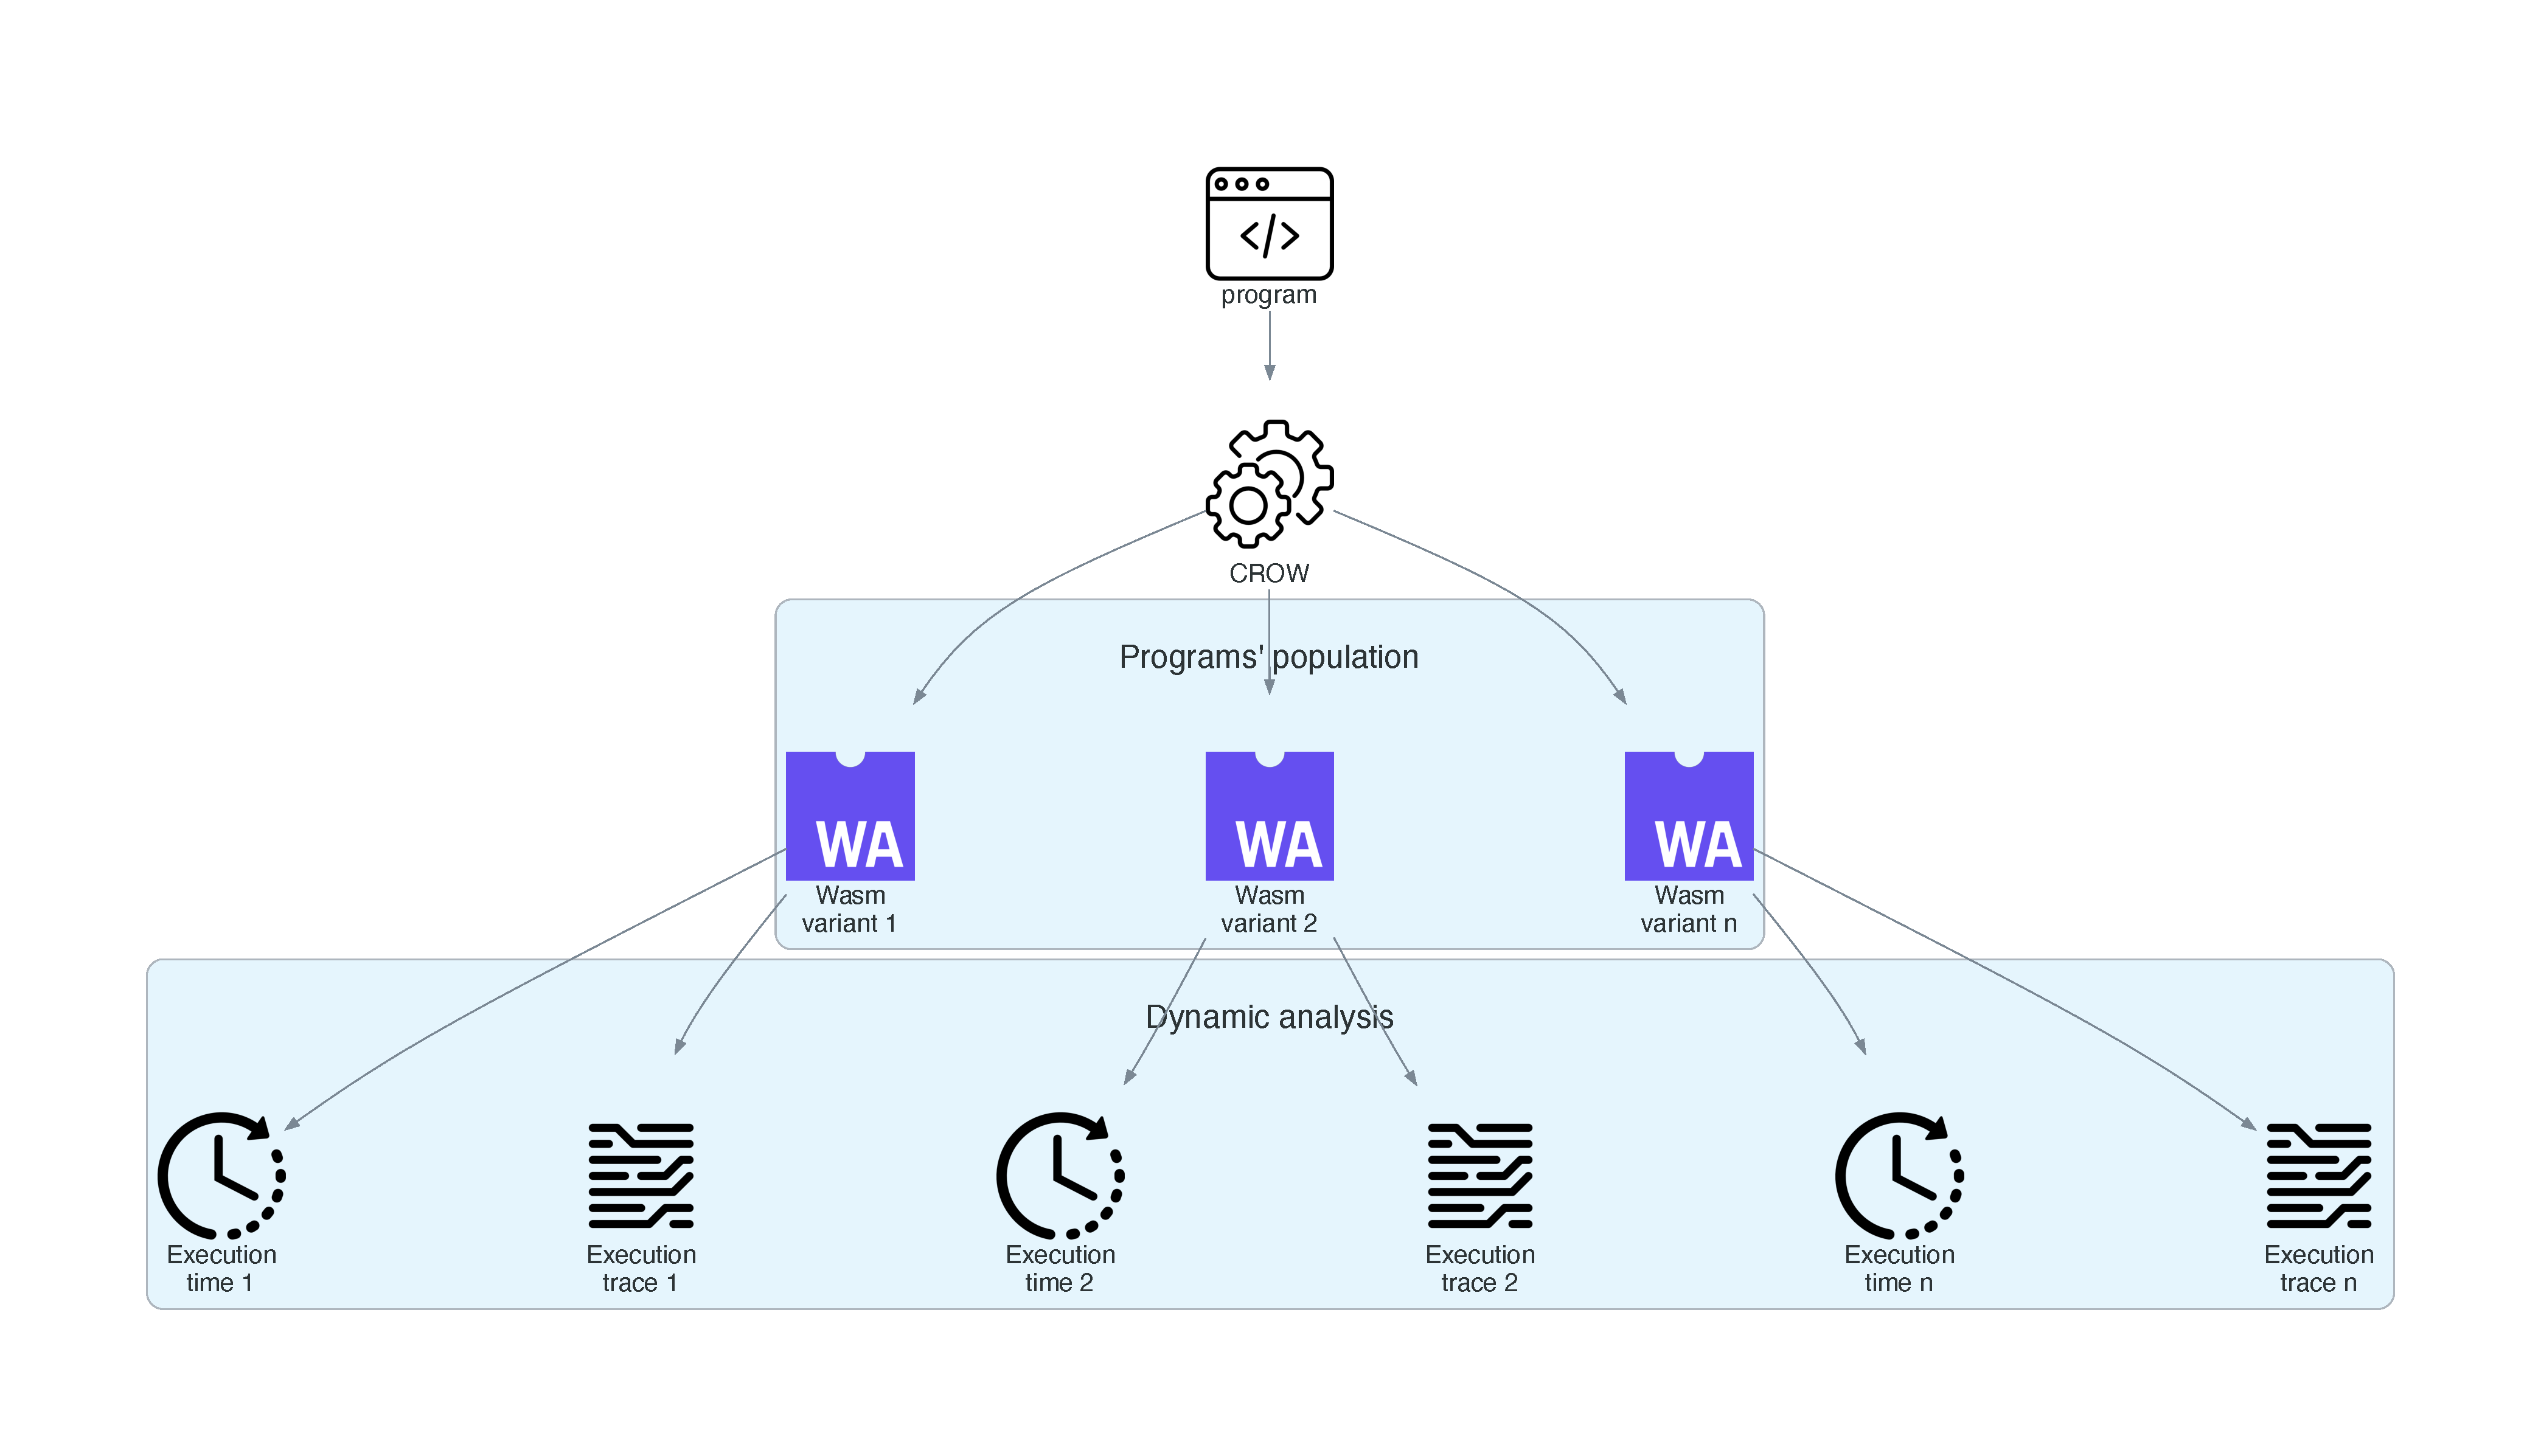
\includegraphics[width=\linewidth]{diagrams/Rq2.pdf}
    \caption{Dynamic analysis for RQ2.}
    \label{diagrams:protocol:rq2}
\end{figure*}

In this second research question, we investigate to what extent the artificially created variants are dynamically different between them and the original program. To conduct this research question, we could separate our experiments into two fields as \autoref{diagrams:protocol:rq2} illustrates: static analysis and dynamic analysis. 
The static analysis focuses on the appreciated differences among the program variants, as well as between the variants and the original program, and we address it in answering RQ1. 
With RQ2, we focus on the last category, the dynamic analysis of the generated variants. This decision is supported because dynamic analysis complements RQ1 and, it is essential to provide a full understanding of diversification.
We use the original functions from \corpusrosetta corpus described in \autoref{section:crow:corpora} and their variants generated to answer RQ1. 
We use only \corpusrosetta to answer RQ2 because this corpus is composed of simple programs that can be executed directly without user interaction, \ie we only need to call the interpreter passing the \wasm binary to it. 

\todo{Motivate, Increasing attack surface does not necesarilly has an impact on defence. For example, reordering instructions for code blocks that are never executed does not impact attacker}

To dynamically compare programs and their variants, we execute each program on each programs' population to collect and execution times. We define execution trace and execution time in the following section.
%\todo{vague and subjective, avoid or elaborate: We perform fine-grained} comparisons by comparing the traces and execution times for all pairs of programs. Therefore, the defined metrics are formulated to support a pairwise comparison strategy.
%In the following, we define the metrics used to answer RQ2.

\subsection*{Metrics}
\label{rq2:metrics}

We compare the execution traces of two any programs of the same population with a global alignment metric. We propose a global alignment approach using Dynamic Time Warping (DTW).
Dynamic Time Warping \cite{NEEDLEMAN1970443} computes the global alignment between two sequences. It returns a value capturing the cost of this alignment, which is a distance metric. The larger the DTW distance, the more different the two sequences are.
DTW has been used for comparing traces in different domains. For software, De A. Maia \etal \cite{ Maia08usinga} proposed to identify similarity between programs from execution traces.
In our experiments, we define the traces as the sequence of the stack operations during runtime, \ie the consecutive list of \texttt{push} and \texttt{pop} operations performed by the \wasm engine during the execution of the program.
In the following, we define the $\DTW$ metric. 
 


\todo{before, define this and give an illutrative listing plus, says how you collect those traces, that's part of the protocol: between the stack operation traces }

\begin{metric}{\DTW{}:}
\label{metric:stack}
\normalfont 
	Given two programs P and P' from the same program's population, \DTW{}(P,P'), computes the DTW distance collected during their execution. \\
	A \DTW{} of $0$ means that both traces are identical.
	The higher the value, the more different the traces. 
\end{metric}



Moreover, we use the execution time distribution of the programs in the population to complement the answer to RQ2. For each program pair in the programs' population, we compare their execution time distributions. We define the execution time as follows:

\begin{metric}{Execution time:}\label{metric:time}
    \normalfont 
	Given a \wasm program P, the execution time is the time spent to execute the binary.
\end{metric}



%\subsection{Variants preservation}

\subsection*{Protocol}

% Dynamic
To compare program and variants behavior during runtime, we analyze all the unique program variants generated to answer RQ1 in a pairwise comparison using the value of aligning their execution traces (\autoref{metric:stack}). We use SWAM\footnote{\url{https://github.com/satabin/swam}} to execute each program and variant to collect the stack operation traces. SWAM is a \wasm interpreter that provides functionalities to capture the dynamic information of \wasm program executions, including the virtual stack operations.
% \todo{Can the reader runderstand that? We want to remark that we only collect the stack operation traces due to the memory-agnosticism of our approach to generate variants. Our approach does not change the memory-like operations of the original code.}

Furthermore, we collect the execution time, \autoref{metric:time}, for all programs and their variants. We compare the collected execution time distributions between programs using a Mann-Withney U test \cite{mann1947} in a pairwise strategy.

%\todo{Maybe the first time that Mann-Withney is mentioned I should describe what it is}

 


\section{\rqthree}
\label{rq3:method}


\todo{The last method is too short}


\newcommand{\mewe}{MEWE\xspace}

\begin{figure}[h]
    \centering
    \includegraphics[width=0.8\linewidth]{diagrams/Rq3.pdf}
    \caption{Multivariant binary creation and workflow for RQ3 answering.}
    \label{diagrams:protocol:rq3}
\end{figure}

In the last research question, we study whether the created variants can be used in real-world applications and what properties offer the composition of the variants as multivariant binaries. \todo{Not defined: We build multivariant binaries}, and we deploy and execute them at the Edge. The process of \emph{mixing} multiple variants into one multivariant binary is an essential contribution of the thesis that is presented in details in \cite{2021arXiv210808125C}. RQ3 focuses on analyzing the impact of this contribution on execution times. To answer RQ3, we use the variants generated for the programs of \corpussodium and \corpusqrcode corpora, we take $2 + 5$ programs interconnecting the LLVM bitcode modules (mentioned in \autoref{table:corpora}). We illustrate the protocol to answer RQ3 in \autoref{diagrams:protocol:rq3} starting from the creation of the programs' population.



%The workflow starts by using the programs' population of each program generated in RQ1 to create the multivariant binaries. We deploy the multivariant binaries at the Edge, and we collect their execution times. We measure the differences for the execution times on the edge. Then, we discuss how multivariant binaries contribute to less predictable timing side-channels.

\subsection*{Metrics}

We use the execution time of the multivariant binaries to answer RQ3. We use the same metric defined in \autoref{metric:time} for the execution time of multivariant binaries.

\subsection*{Protocol}


We run the experiments to answer RQ3 on the Edge, \todo{too fast. tell the reader why you need HTTP now: executing the multivariant binaries as end-to-end HTTP services.} 
The execution times are measured at the backend space, \ie we collect the execution times inside the Edge node and not from the client computer. Therefore, we instrument the binaries to return the execution time as an HTTP header. We do this process for the original program and its multivariant binary. We deploy and execute the original and the multivariant binaries on 64 edge nodes located around the world \todo{Add illustrative map}.


We collect 100k execution times for each binary \todo{Why? Cite blackhat paper and the need of 1 million traces multiplied by the number of nodes}, both the original and multivariant binaries.
We perform a Mann-Withney U test \cite{mann1947} to compare both execution time distributions. 
If the P-value is lower than 0.05, the two compared distributions are different.

%\pagebreak

\section{Conclusions}

This chapter presents the methodology we follow to answer our three research questions. We first describe and propose the corpora of programs used in this work. We propose to measure the ability of our approach to generate variants out of \py{303  + \libsodiumfunctions + \qrcodefunctions} functions of our corpora. Then, we suggest using the generated variants to study to what extent they offer different observable behavior through dynamic analysis. We propose a protocol to study the impact of the composition variants in a multivariant binary deployed at the Edge. Nevertheless, we enumerate and enunciate the properties and metrics that might lead us to answer the impact of automatic diversification for \wasm programs. In the next chapter, we present and discuss the results obtained with this methodology.

\clearpage